\documentclass{article}
\usepackage[margin=1in]{geometry} %1 in margins
\usepackage{graphicx} %For including graphics
\usepackage[labelfont=bf]{caption} %Make float labels bold
\usepackage{subcaption}
\usepackage{amsmath}    
\usepackage{listings}% http://ctan.org/pkg/listings
\lstset{
  basicstyle=\ttfamily,
  mathescape
}
\usepackage{hyperref}
\renewcommand{\floatpagefraction}{0.95}
\renewcommand{\topfraction}{0.95}
\renewcommand{\textfraction}{0.05}
\usepackage{url}

% Define a ``Program'' float for code
\usepackage{verbatim} %Allow verbatim input for code
\usepackage{float} %Defining the Program environment
\floatstyle{boxed}
\newfloat{program}{htbp}{pgm}
\floatname{program}{Program}
\usepackage[fontsize=9pt]{scrextend}
\usepackage{color,soul}



\begin{document}

\begin{flushright}
Mehmet Duman
\end{flushright}

\begin{center}
{\Large {\bf Solution to Homework \#4---EAS 520 \& DSC 520 \& MTH 499} }
\end{center}

{\bf Problem 1}




\begin{center}
$I = \int_{R} f(x) dx, $
\end{center}
by Monte Carlo integration
\begin{equation} \label{exp:eq0}
I = V  \frac{1} {N}  \displaystyle\sum_{i=1}^{ N} f(x_i)					
\end{equation}

\begin{center}
	$V = \int_{R} dx, $
\end{center}
Monte Carlo integration algorithm implement in C and program accept N as an input and output the approximate value  (\textcolor{red}{1}). Your program should work for any function $\mathcal{L}$. Your program should also output the intermediate values of $\hat{I}(i)$ (the approximate value of the integral using i random samples) after every $i = 4^k$ iterations, where k = 2, 3, 4, 5, . . . . For example, if you let N = 256, your code should output the approximate value of the integral after 16,64,256 iterations.  Test your code on a case of;
\begin{equation} \label{exp:eq0}
\mathcal{L}(x_1,x_2,x_3,x_4,x_5,x_6,x_7,x_8,x_9,x_{10})=x_1 +x_2 +x_3 +x_4 +x_5 +x_6 +x_7 +x_8 +x_9 +x_{10}, 
\end{equation}
Provide evidence that your code is working by showing the Monte Carlo estimate of the integral is converging to 0.
\\
\\
NOTE:Because the volume term V is going to be very large, so instead of (or in addition to) looking at the convergence of the integral, you can compute the Monte Carlo approximation of:
\begin{equation} \label{exp:eq0}
\frac{1} {V}  \int_{R} \mathcal{L}(x) d^{10}x, 
\end{equation}

Use OpenMP to parallelize the for-loop over the number of random samples. That is, each thread should make independent random draws, independently evaluate $\mathcal{L}(x)$ at the random value, and update the sum. For full credit, your program must continue to output the integral’s value approximately every $i = 4^k$ iterations, where k = 2,3,4,5...
Rerun the test given in (\textcolor{red}{2}) to show the code still works when using 4 threads. Use OpenMP routines to explicitly output the number of threads that are being used and provide evidence that the number of threads is indeed 4.
\\
\\

{\bf Problem 2}

\begin{equation} \label{exp:eq0}
| \hat{I}(4^k) - \hat{I} | \approx  | \hat{I}(4^k) - \hat{I}(4^{k+1}) | 
\end{equation}


Add the error estimator Eq.(3) to your OpenMP code. That is, have your code output the value $|\hat{I}(4^k)-\hat{I}(4^{k+1})|$ 
along with the value of the integral $ \hat{I}(4^k) $.

Rerun the test Eq.(3). Plot both the actual error,   $ | \hat{I}(i) - 0 | $ , versus i and the estimated error versus i on 
the same figure. Consider up to large values of i.
\\
\\
\\
\\
\textbf{\textit{Solution for Problem 1 and Problem 2}} :
\\
\\
Below is an example C program that accept N (iterations) and dim (function dim-dimensional )  as input and output  approximate value of Monte Carlo integration from given by Eq: (\textcolor{red}{2}) the integral Eq:(\textcolor{red}{3}). The program sets the seed base on current time (srand(time(NULL))). That way, when we call rand() function we will get random numbers between [a,b] which we  use to calculate function Eq:(\textcolor{red}{2}) and than we apply integral Eq:(\textcolor{red}{1}) for approximation. As we can see from following approximate integral data for hw4\_p1b.txt, the integral is converging to 0 

\newpage

\begin{program}
	\begin{verbatim}
#include <stdlib.h>
#include <stdio.h>
#include <time.h>
#include <math.h>
double sample_interval(double a, double b) {
   double x = ((double) rand())/((double) RAND_MAX);
   return (b-a)*x + a; }

double funcL(double array[], int rows) {
   double L = 0.0;
   for (int j=0; j < rows; ++j) {
      L += array[j]; }
   return L; }

int main (int argc, char **argv) {
   srand(time(NULL));
   int dim = atoi( argv[1] );           // convert command-line input to dim = number of dimensions
   unsigned long long int N = atoll( argv[2] ); // convert command-line input to N= number of points
   double xdim[dim];
   double a = -5.0, b =  5.0;
   long int V = 1;
   for (int m=1; m <= dim; ++m) {
      V *= (b-a);  }
   double integral = 0.0;
   unsigned long long int p_pow = 16;

   for (unsigned long long int i=0; i < N; ++i) {
      for (int k=0; k < dim; ++k) {
         xdim[k] =sample_interval( a,b );
      }
      integral += funcL( xdim, dim );
      if ( i == p_pow ) {
         printf("Dimensions= %i, iterations= %10llu, Z= % 3.12e\n",
            dim, i, (double)V * integral/ ( (double)i * (double)V) );
         p_pow *= 4;
      }
   }
   printf("Dimensions= %i, iterations= %10llu, Z= % 3.12e\n",
      dim, N, (double)V * integral/ ( (double)N * (double)V) );
   return 0;
}
	\end{verbatim}
	\caption{The C program for generate  Monte Carlo approximation.}
\end{program}


The C program generated following txt files: 
\begin{lstlisting}
>>> ./hw4_p1b 10 100000000 > hw4_p1b.txt          
\end{lstlisting}
\begin{lstlisting}
Dim= 10, iterations=         16, Z= -3.466072939204e-01
Dim= 10, iterations=         64, Z=  7.198029258584e-01
Dim= 10, iterations=        256, Z=  7.428388387601e-01
Dim= 10, iterations=       1024, Z=  2.193662219927e-01
Dim= 10, iterations=       4096, Z=  9.710737150246e-02
Dim= 10, iterations=      16384, Z= -2.108062003019e-02
Dim= 10, iterations=      65536, Z= -1.900207465166e-02
Dim= 10, iterations=     262144, Z= -1.651675140169e-02
Dim= 10, iterations=    1048576, Z= -2.861002458223e-03
Dim= 10, iterations=    4194304, Z= -2.120815241001e-03
Dim= 10, iterations=   16777216, Z=  6.045395321028e-04
Dim= 10, iterations=   67108864, Z=  3.448560390746e-04
Dim= 10, iterations=  100000000, Z=  6.747072587884e-04
\end{lstlisting}




\newpage
Below is an example program that use OpenMP to parallelize the for-loop over the number of random samples. Each thread make independent random draws, independently evaluate  $\mathcal{L}(x)$ at the random value, and update the sum. This program  continues to output the integral value approximately every $i = 4^k$ iterations, where 
\\
k = 2,3,4,5.... End of the each $4^k$ iterations, one of the threads output approximates MC integral value.
\\
\\
Error estimator Eq. (\textcolor{red}{4}) has been added to the code and the code outputs the value $|\hat{I}(4^k)-\hat{I}(4^{k+1})|$ 
along with the value of the integral $ \hat{I}(4^k) $.
\\
\\
Below program uses the  Eq:(\textcolor{red}{4})  and  Eq:(\textcolor{red}{3}) to calculate MC approximation.   

\begin{figure}[htb]
	\begin{center}
		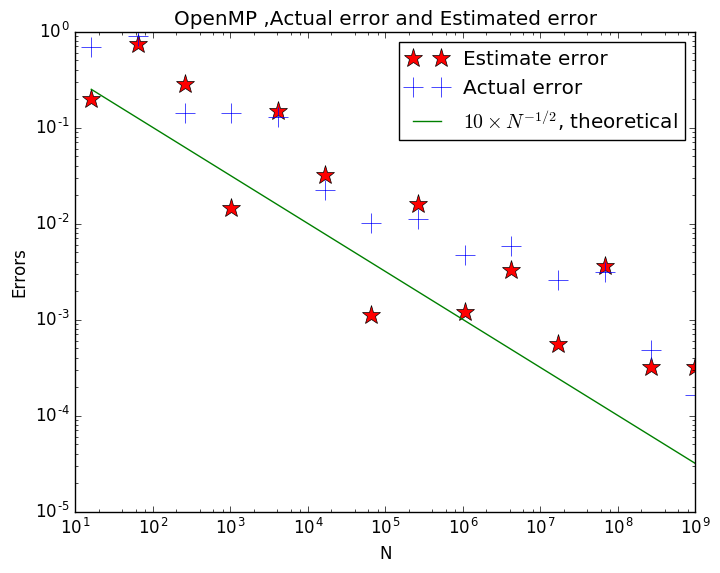
\includegraphics[width=0.8\textwidth]{hw4_p2b.png}
	\end{center}
	\caption{Errors versus Iterations. Data has been generated by C code below and plot by python-matplotlib }
	\label{fig:hw4_p2b}
\end{figure}



\begin{program}
	\begin{verbatim}
	#include <stdlib.h>
	#include <stdio.h>
	#include <stdbool.h>
	#include <time.h>
	#include <math.h>
	#include <omp.h>
	double sample_interval(double a, double b) {     // Random Numbers generation beteeen (a,b)
	  double x = ((double) rand())/((double) RAND_MAX);
	  return a + (b-a)*x ;  }
	double funcL(double array[], int rows) {          // Function L(x1 +x2 +...+xj)
	  double L = 0.0;
	  for (int j=0; j < rows; ++j) {
	    L += array[j];  }
	  return L;  	}

	int main (int argc, char **argv) {
	  srand(time(NULL));
	  int dim = 10
	  unsigned long long int N = atoll( argv[1] );               // atoll for long numbers: iterations
	  double xdim[dim];
	  double a = -5.0, b =  5.0 ;
	//    long int V = 1;                                       // Volume,but ignored  applying MC appr
	//    for (int m=1; m <= dim; ++m) { V *= (b-a);  }
	  int pow_max = 0;
	  do {
	    pow_max += 1;
	  } while (pow(4, pow_max)  < N);                            // Find closest power of 4 to  N value
	  double approx_integral[pow_max]  ;                         //  to save integral values of 4^k iter
	  double integral      = 0.0;
	  double err_estimator = 0.0;
	  int pow_count = 2;                                         // For first number  16 = 4^2
	  unsigned long long int n_start =  1;
	  unsigned long long int n_stop  = 16;
	  bool working_loop = true;
      long long int n;
	  do {
	    if (n_stop > N ) {                                      // Check n_stop if it is bigger than N
	      n_stop = N;                                           // change it with N for loop
	      working_loop = false;  }                              // exit from while loop endofthe circle
	    #pragma omp parallel for private(xdim) reduction(+: integral) num_threads(4)    // OMP START
	    for (int n = n_start ; n <= n_stop ; n+=1) {            // Iteration between 4^k - $^k+1 
	      int i;
	      for ( i=0; i < dim; ++i) {
	        xdim[i] =sample_interval( a,b );                    // Genarate 'dim' number between (a,b)
	      }
	      integral += funcL( xdim, dim );                       // Apply funcL and add it up integral 
	    }                                                       // PARALLEL COMPUTING END
	    approx_integral[pow_count] = integral/ (double)n_stop ; // Calc integral 'pow_count' iteration
	    pow_count += 1;                                         // prepare 'pow_count' for next iteratin
	    n_start    = n_stop+1;                                  // prepare n_start for next for loop
	    n_stop     *= 4 ;                                       // n_stop for next for loop by mltiply*4
	  } while ( working_loop );
	
	  n_stop = 4;	
	  for (int i=2; i < pow_max ; ++i) {                        // print approx MC  and error for 4^k
	    n_stop *= 4;
	    printf(" %16llu,% 3.16e,%3.16e,%3.16e \n", n_stop, approx_integral[i], 
	         fabs(approx_integral[i] - approx_integral[i+1]), fabs(approx_integral[i] - 0.0) );
	  }
	printf(" %16llu,% 3.16e,%3.16e,%3.16e  \n" ,                // print approx MC  for N iteration
	     N, approx_integral[pow_max], fabs(approx_integral[pow_max] - approx_integral[pow_max-1]),
	     fabs(approx_integral[pow_max] - 0.0) );
	return 0;  }
		\end{verbatim}
	\caption{The C program use OpenMP to parallelize the for-loop to generate  Monte Carlo approximation}
	\label{fig:hw4_p1c}
\end{program}

\newpage

Below Python program reads the text files which is created by C code above and plot both the actual error,   $ | \hat{I}(i) - 0 | $, versus i and the estimated error versus i on the same figure. 
It is implemented in Python, and makes use of the NumPy and matplotlib packages.
\begin{program}
	\begin{verbatim}
	import numpy as np
	from matplotlib import pyplot as plt
	
	def Homework4_p2(path, data_filenames):
	   	### import data ###
	   	data = np.loadtxt(path+data_filenames+'.txt', delimiter=',', usecols=range(4))
	   	### plot results ###
	   	fig = plt.figure()
	   	plt.loglog(data[:,0],data[:,2],'r*',markersize=14,label='Estimate error')
	   	plt.loglog(data[:,0],data[:,3],'b+',markersize=14,label='Actual error')
	   	
	   	plt.legend()
	   	plt.xlabel('N Iterations')
	   	plt.ylabel('Errors')
	   	plt.title('Compare Actual error and Estimated error')
	   	plt.savefig(path+data_filenames+'.png' , bbox_inches='tight')
	   	return
	   		
	def run():    
	   	path = "/Users/ekinezgi/Documents/UmassD/DSC520/umassd-hpc-mehmetduman/HW4/"
	   	fnames_p2b = "hw4_p2b"
	   	Homework4_p2(path,fnames_p2b) 
	   	return
	   		
	if __name__ == '__main__':
	   run()
	\end{verbatim}
	\caption{The Python program used to generate Fig.\ \ref{fig:hw4_p2b}.}
\end{program}


Below tex files (hw4\_p2b.txt)  generated by C Program:\ref{fig:hw4_p1c} (hw4\_p1c.c) and used by above python program to generate Figure:\ref{fig:hw4_p2b} 
\begin{lstlisting}
>>> ./hw4_p1c 10 1000000000 >  hw4_p2b.txt
               16, 6.8952377510234886e-01,1.9873449653619202e-01,6.8952377510234886e-01 
               64, 8.8825827163854087e-01,7.4653673906343743e-01,8.8825827163854087e-01 
              256, 1.4172153257510342e-01,2.8392992476289891e-01,1.4172153257510342e-01 
             1024,-1.4220839218779552e-01,1.4678971920162265e-02,1.4220839218779552e-01 
             4096,-1.2752942026763325e-01,1.4975651530658102e-01,1.2752942026763325e-01 
            16384, 2.2227095038947760e-02,3.2315206043078637e-02,2.2227095038947760e-02 
            65536,-1.0088111004130873e-02,1.1172354111771803e-03,1.0088111004130873e-02 
           262144,-1.1205346415308053e-02,1.5862429979521836e-02,1.1205346415308053e-02 
          1048576, 4.6570835642137844e-03,1.1897692194518085e-03,4.6570835642137844e-03 
          4194304, 5.8468527836655930e-03,3.2442244809695931e-03,5.8468527836655930e-03 
         16777216, 2.6026283026959998e-03,5.6075020141608785e-04,2.6026283026959998e-03 
         67108864, 3.1633785041120877e-03,3.6486997125633937e-03,3.1633785041120877e-03 
        268435456,-4.8532120845130617e-04,3.2317370239185708e-04,4.8532120845130617e-04 
       1000000000,-1.6214750605944911e-04,3.2317370239185708e-04,1.6214750605944911e-04  

\end{lstlisting}




The OpenMP C Program:\ref{fig:hw4_p1c} (hw4\_p1c.c)  modified to print out thread info inside the for-loop to show how many threads being used. This is the evidence that the number of threads is indeed 4.
\begin{verbatim}
$ ./hw4_p1c 20 
\end{verbatim}

\begin{lstlisting}
>>> ./hw4_p1c 10 20 
iteration=      5, thread = 1,  n_start= 1,n_stop= 16, thread_integral_sum=  2.076520510984829 
iteration=      9, thread = 2,  n_start= 1,n_stop= 16, thread_integral_sum=  3.160693623666042 
iteration=     13, thread = 3,  n_start= 1,n_stop= 16, thread_integral_sum=  8.018336770133272 
iteration=      1, thread = 0,  n_start= 1,n_stop= 16, thread_integral_sum=  18.472768859226619 
iteration=      6, thread = 1,  n_start= 1,n_stop= 16, thread_integral_sum=  15.957093986662613 
iteration=     10, thread = 2,  n_start= 1,n_stop= 16, thread_integral_sum= -3.913657811430124 
iteration=     14, thread = 3,  n_start= 1,n_stop= 16, thread_integral_sum=  0.775044798280599 
iteration=      2, thread = 0,  n_start= 1,n_stop= 16, thread_integral_sum=  15.273116610605793 
iteration=      7, thread = 1,  n_start= 1,n_stop= 16, thread_integral_sum=  26.838730795699512 
iteration=     11, thread = 2,  n_start= 1,n_stop= 16, thread_integral_sum=  4.827635569883338 
iteration=     15, thread = 3,  n_start= 1,n_stop= 16, thread_integral_sum=  11.179546323222826 
iteration=      3, thread = 0,  n_start= 1,n_stop= 16, thread_integral_sum=  29.485163269324772 
iteration=      8, thread = 1,  n_start= 1,n_stop= 16, thread_integral_sum=  42.286921535752207 
iteration=     12, thread = 2,  n_start= 1,n_stop= 16, thread_integral_sum= -5.913969434757705 
iteration=     16, thread = 3,  n_start= 1,n_stop= 16, thread_integral_sum=  20.680923820790326 
iteration=      4, thread = 0,  n_start= 1,n_stop= 16, thread_integral_sum=  20.046715764350594 

iteration=     16, thread = 0, total_integral_sum=  77.100591686135431, 
***approx MC integral=  4.818787e+00 

iteration=     18, thread = 1,  n_start= 17,n_stop= 20, thread_integral_sum= -6.401136636920802 
iteration=     19, thread = 2,  n_start= 17,n_stop= 20, thread_integral_sum=  1.911123391199451 
iteration=     20, thread = 3,  n_start= 17,n_stop= 20, thread_integral_sum=  7.367492358837044 
iteration=     17, thread = 0,  n_start= 17,n_stop= 20, thread_integral_sum= -6.572933307184341 

iteration=     20, thread = 0, total_integral_sum=  73.405137492066785, 
***approx MC integral=  3.670257e+00 


16, 4.8187869803834644e+00,1.1485301057801252e+00,4.8187869803834644e+00 
20, 3.6702568746033393e+00,1.1485301057801252e+00,3.6702568746033393e+00  

\end{lstlisting}
.
\newline
\\
{\bf Problem 3a, 3b, 3c, 3d}

Modify your OpenMP parallelized code to let

\begin{equation} \label{exp:eq0}
\mathcal{L}(x_1,x_2,x_3,x_4,x_5,x_6,x_7,x_8,x_9,x_{10})= exp( - \displaystyle\sum_{i=1}^{ 9} [ (1-x_i)^2 + 100(x_{i+1}-x_i^2)^2 ] ) ,
\end{equation}

which is the higher dimensional extension of the 2-dimensional function you used in homework 3. What’s the value of this integral when N = 1024 = 45 = 210 (sampling about 2 points per dimension)? With so few points, the value should be far from the true value.

Read up on OpenMP’s function omp get wtime() and use this to measure the code’s so-called walltime. You want to call the timer at the very beginning and at the very end of the program.

Run your code on Stampede using a single compute node (submit with sbatch). Let N = 106 and com- pute the code’s speedup using 1, 2, 4, 8 and 16 threads. Your timing measurement should use the function omp get wtime(). Plot the number of threads versus speedup. This is called a strong scaling test: you keep the problem sized fixed (you hold N constant) and let the number of threads increase.

Run your code on Stampede using a single compute node (submit with sbatch). Let N = threads × 105 and compute the code’s speedup using 1, 2, 4, 8 and 16 threads. Your timing measurement should use the function omp get wtime(). Plot the number of threads versus speedup. This is called a weak scaling test: you let the problem size N increase with the number of cores.
\\
\\
\textbf{\textit{Solution for Problem 3a, 3b, 3c, 3d}} :
\\
Below is an example C program that accept threads\_tot (total number of treads want to use), N (iterations) and dim (function dim-dimensional )  as an input and output  to approximate the value of Monte Carlo integration from given by Eq:(\textcolor{red}{5}) the integral

\begin{equation} \label{exp:eq0}
 \mathcal{Z}=  \int_{R} \mathcal{L}(x) d^{10}x, 
\end{equation}

Program sets the seed base on current time (srand(time(NULL) * omp\_get\_thread\_num()  )). That way, when we call rand() function, we will get random numbers between [a,b] which we use to calculate function Eq:(\textcolor{red}{5}) and than we apply MC approximation for Eq:(\textcolor{red}{6}).

\begin{program}
	\begin{verbatim}
#include <stdlib.h>, #include <stdio.h>, #include <stdbool.h>, #include <time.h>
#include <math.h>, #include <omp.h>, #include <sys/time.h>
double sample_interval( double a, double b) {     // Random Numbers generation beteeen (a,b)
  double x = (double)rand() / RAND_MAX;
  return a + (b-a)*x ;   }
double funcL(double array[] ) {
  double L = 0.0;
  for (int j=0; j < 9; ++j) {
    L += ( 1.0 - array[j] )*( 1.0 - array[j] ) + 
           100.0 * ( array[j+1] - array[j] * array[j] ) * ( array[j+1] - array[j] * array[j] ) ; }
  return exp( -1.0 * L );  }

int main (int argc, char **argv) {
  double start_time = omp_get_wtime();
  srand(time(NULL) * omp_get_thread_num() );
  const int dim =  10;
  int threads_tot = atoi( argv[1] );
  int threads_check;

  bool working_loop = true;
  unsigned long long int N = atoll( argv[2] );  // atoll for long numbers:
  if ( isinf(N) || N == 0 || N == 705032704 || N == 9223372036854775807) {   
    printf(" N is too big ... INFINITY \n");
    working_loop = false;    }                                 

  double xdim[dim], a = -0.5, b =  0.5, double V = 1.0;                         
  for (int m=1; m <= dim; ++m) {
    V *= (b-a);   }

  int pow_max = 0;
  do {
    pow_max += 1;
  } while (pow(2, pow_max)  < N);         // Find out closest power of 4 to input N value

  double funcL_sum      = 0.0;
  int pow_count = 1;
  unsigned long long int n_start = 1;
  unsigned long long int n_stop  = 2;
  unsigned long long int n;

  while ( working_loop ) {
  if (n_stop >= N || isinf(n_stop) || n_stop == 0 ) {                // n_stop*4 =0 when it is inf
    n_stop = N;                                                       // change it with N for loop
  working_loop = false;                                                    // exit from while loop 
  }

  #pragma omp parallel for private(xdim) reduction(+: funcL_sum) num_threads(threads_tot)  // START
  for ( n = n_start ; n <= n_stop ; n+=1) {                  // Iteration between each power of 2 
    int i;
    for ( i=0; i < dim; ++i) {
      xdim[i] = sample_interval( a,b );                      // Genarate 'dim' number between (a,b)
    }
    funcL_sum += funcL( xdim );                     // Apply func L and add it up integral veriable
    threads_check = omp_get_num_threads();
  }                                                                      // PARALLEL COMPUTING END

  printf(" %16llu,% 3.16e \n", n_stop, V * funcL_sum/ (double)n_stop );
  pow_count += 1;
  n_start    = n_stop+1;                                        // prepare n_start for next for loop
  n_stop    *= 2 ;                                  // prepare n_stop for next for loop by multipl 4
}
double finish_time = omp_get_wtime();
printf("%i, %f ,%f ,%f\n", threads_check, (finish_time - start_time), start_time, finish_time);
return 0;  }
	\end{verbatim}
	\caption{For Problme 3a: MC approximation for eq.(\textcolor{red}{6}) }
	\label{fig:hw4_p3abcd}
\end{program}																								 

\newpage


The upper  C Program:\ref{fig:hw4_p3abcd}(hw4\_p3abcd.c) generate following hw4\_p3abcd\_7821842.stdoudata files on Stampede:
\begin{lstlisting}
                2, 6.0266666418308394e-26 
                4, 3.0133359225397913e-26 
                8, 2.2428399699822230e-23 
               16, 1.1214207772078482e-23 
               32, 1.9621276583651485e-21 
               64, 3.7362519348866332e-14 
              128, 1.4574964659143308e-11 
              256, 7.2874891432678335e-12 
              512, 3.6694483193548139e-12 
             1024, 1.8591279039282411e-12 

        16, 0.037607 ,694709.841734 ,694709.879341
\end{lstlisting}



I modified above C Program  \ref{fig:hw4_p3abcd} to get speed of program and generated two text files on Stampede (Data information is below Figure"\ref{fig:hw4_p3c_7822316} ). First file is  for Strong Scalling Test and second file is for Weak Scalling test.

The below python program use those two text files, to calculate Speedup and plot the Scalling Test on the same figure. 
It is implemented in Python, and makes use of the NumPy and matplotlib packages.

\begin{program}
	\begin{verbatim}
import numpy as np
from matplotlib import pyplot as plt
def Homework4_p3c(path, data_filenames, data_filenames_2):
    ### import data ###
    data = np.loadtxt(path+data_filenames+'.stdou', delimiter=',', usecols=range(4))
    data_2 = np.loadtxt(path+data_filenames_2+'.stdou', delimiter=',', usecols=range(4))
    ### Spedup Calculation #############
    # For spedup I used  http://stackoverflow.com/questions/7925510/parallel-speedup-with-openmp
    # equential time measurement: seq_time = endTime-startTime;
    # Parallel time measurement : paralleltime = endTime-startTime; 
    # speedup = seq_time/paralleltime;
    seq_time = data[0,1] 
    new_col = np.zeros((len(data), 1))
    for i,j in  enumerate(data):
	    new_col[i] = seq_time / data[i,1]
    data = np.c_[data, new_col]
    seq_time = data_2[0,1] 
    new_col = np.zeros((len(data_2), 1))
    for i,j in  enumerate(data_2):
    new_col[i] = seq_time / data_2[i,1]
    data_2 = np.c_[data_2, new_col]
    ### plot results ###
    fig = plt.figure()
    plt.plot(data[:,0],data[:,1],'r*',markersize=20,label='Strong Scaling Test')
    plt.plot(data_2[:,0],data_2[:,1],'bo',markersize=8,label='Weak Scaling Test')
    plt.legend(loc='upper left')
    plt.xlabel('Threads')
    plt.ylabel('Speedup')
    plt.title('OpenMP ,scaling test')
    plt.savefig(path+data_filenames+'.png' , bbox_inches='tight')
    return
	\end{verbatim}
	\caption{The Python program used to generate Fig.\ \ref{fig:hw4_p3c_7822316}.}
	\label{fig:python1}
\end{program}

\newpage
.

\begin{figure}[htb]
	\begin{center}
		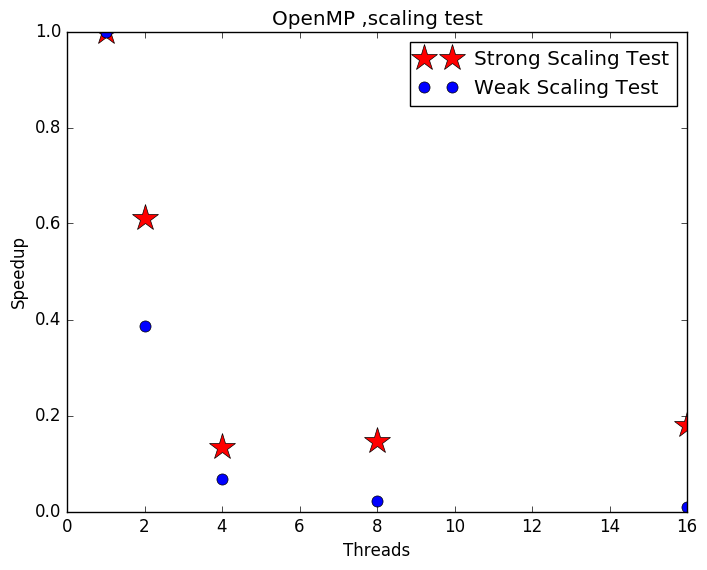
\includegraphics[width=0.8\textwidth]{hw4_p3c_7822316.png}
	\end{center}
	\caption{Stampede Output}
	\label{fig:hw4_p3c_7822316}
\end{figure}


Data for Fig.\ \ref{fig:hw4_p3c_7822316}  which is created by C Program \ref{fig:hw4_p3abcd} above on Stampede. Speedup calculation and plot made by python Program \ref{fig:python1}. 

Strong Scaling Test output files hw4\_p3c\_7822316.stdou: 
\begin{lstlisting}
    N      threads  omp_get_wtime()      start           end           Speedup        
1000000,	  1,	 0.256625 ,	703324.758038 ,703325.014663 ,1.00000000e+00
1000000,	  2,	 0.420077 ,	703324.758083 ,703325.178160 ,6.10899906e-01
1000000,	 16,	 1.420244 ,	703324.758068 ,703326.178311 ,1.80690783e-01
1000000,	  8,	 1.756162 ,	703324.758026 ,703326.514188 ,1.46128318e-01
1000000,	  4,	 1.902061 ,	703324.758113 ,703326.660174 ,1.34919437e-01
\end{lstlisting}


Weak Scaling Test output files hw4\_p3c\_7822321.stdou: 
\begin{lstlisting}
      N  threads   omp_get_wtime()      start            end           Speedup        
 100000,	 1,	 0.039437 ,	698939.339748 ,	698939.379185, 1.00000000e+00
 200000,	 2,	 0.102246 ,	698939.339756 ,	698939.442002, 3.85707020e-01
 400000,	 4,	 0.576559 ,	698939.339819 ,	698939.916378, 6.84006320e-02
 800000,	 8,	 1.837545 ,	698939.339870 ,	698941.177415, 2.14617873e-02
1600000,	 16,	 4.221020 ,	698939.339775 ,	698943.560794, 9.34300240e-03
\end{lstlisting}


.
\newpage

{\bf Problem 3e}
\\
The goal of this last part is to attempt to compute the integral (2), with the likelihood function L given by Eq. (7), to about 1 digit of accuracy. This may be difficult. In fact this problem comes from a recently published research paper and so we (the class) are trying to reproduce their published result. Please post any issues or difficulties you encounter on Piazza. Hopefully we can reproduce their result! Run your code on stampede using 16 threads. Plot i vs I(i) on a semilogx plot. Also plot i vs the estimated error. You can continue to output
every i = 4k iterations, where k = 2, 4, 5, . . . , as well as outputting the final value computed using all N points. Go to as high of a value of N (with N being “unsigned long long int” if necessary) as you need to compute the integral to 1 digit of accuracy. Use your error estimator to inform you of the accuracy. From your data, what do you think is the integral’s value and how accurate is its value?
\\
\\
\textbf{\textit{Solution for Problem 3e}} :
\\
Program sets the seed base on current time (srand(time(NULL) * omp\_get\_threa\_num() )). That way, when we call rand() function we will get random numbers between [a,b] which we are using to calculate function Eq:(\textcolor{red}{5}) and than we apply MC approximation for  Eq:(\textcolor{red}{6}).



\begin{program}
	\begin{verbatim}
#include <stdlib.h>, #include <stdio.h>, #include <stdbool.h>, #include <time.h>
#include <math.h>, #include <omp.h>, #include <sys/time.h>
double sample_interval( double a, double b) {     // Random Numbers generation beteeen (a,b)
  double x = (double)rand() / RAND_MAX;
  return a + (b-a)*x ;  }
double funcL(double array[] ) {
  double L = 0.0;
  for (int j=0; j < 9; ++j) {
    L += ( 1.0 - array[j] )*( 1.0 - array[j] ) + 
      100.0 * ( array[j+1] - array[j] * array[j] ) * ( array[j+1] - array[j] * array[j] ) ;  }
  return exp( -1.0 * L );   }

int main (int argc, char **argv) {
  srand(time(NULL) * omp_get_thread_num() );
  const int dim =  10;
  int threads_tot = atoi( argv[1] );

  bool working_loop = true;
  unsigned long long int N = atoll( argv[2] );                            // atoll for long numbers
  if ( isinf(N) || N == 0 || N == 705032704 || N == 9223372036854775807) {  //70...u int,92..ull int
    printf(" N is too big ... INFINITY \n");
    working_loop = false;        }                                      // exit from while loop end

  double xdim[dim], a = -0.5, b =  0.5, V = 1.0;                                 
  for (int m=1; m <= dim; ++m) {													
    V *= (b-a);  }	                                                                   // For Volume

  int pow_max = 0;
  do {
    pow_max += 1;
  } while (pow(4, pow_max)  < N);                   // Find out closest power of 4 to input N value

  double funcL_sum      = 0.0;
  int pow_count = 2;                                                  // For first number  16 = 4^2
  unsigned long long int n_start = 1;
  unsigned long long int n_stop  = 16;
  unsigned long long int n;

  while ( working_loop ) {
  if (n_stop > N || isinf(n_stop) || n_stop == 0 ) {                 // n_stop*4 =0 when it is inf   
    n_stop = N;                                                       // change it with N for loop
    working_loop = false;        }                         // exit from while loop end of the circle

  #pragma omp parallel for private(xdim) reduction(+: funcL_sum) num_threads(threads_tot)  // START
  for ( n = n_start ; n <= n_stop ; n+=1) {                    // Iteration between each power of 4
    int i;
    for ( i=0; i < dim; ++i) {
      xdim[i] = sample_interval( a,b );                      // Genarate 'dim' number between (a,b)
    }
    funcL_sum += funcL( xdim );                       // Apply func L and add it up integral veriable
  }                                                                       // PARALLEL COMPUTING END

  printf(" %16llu,% 3.16e \n", n_stop, V * funcL_sum/ (double)n_stop );

  pow_count += 1;
  n_start    = n_stop+1;                                        // prepare n_start for next for loop
  n_stop    *= 4 ;                                 // prepare n_stop for next for loop by multipl 4
}
return 0; }
	\end{verbatim}
	\caption{The C program Stampede outputs for MC approx for L functions hw4\_p3e9\_7820263.stdou Fig.\ \ref{fig:hw4_p3e9_7820263}.}
	\label{fig:hw4_p3e9}
 \end{program}																								 

\newpage


Below Python program read the text files which is created by C Program: \ref{fig:hw4_p3abcd} on Stampede system and calculate estimated error. Program  plot the MC approximation and estimated error. 
It is implemented in Python, and makes use of the NumPy and matplotlib packages.
\begin{program}
	\begin{verbatim}
  import numpy as np
  from matplotlib import pyplot as plt

  def Homework4_p3e(path, data_filenames):
    ### import data ###
    data = np.loadtxt(path+data_filenames+'.stdou', delimiter=',', usecols=range(2))
    ### For Estimated Error Calculation #############
    new_col = np.zeros((len(data), 1))
    for i in range(len(data)-2,-1,-1):
        new_col[i] = abs(data[i,1] - data[i+1,1])

    new_col[len(data)-1] = new_col[len(data)-2] 
    data = np.c_[data, new_col]
    ### plot results ###
    fig = plt.figure()
    ax1 = fig.add_subplot(211)
    ax1.semilogx(data[:,0],data[:,1],'r*',markersize=16,label='$\mathcal{L}$ Approximation')
    ax1.legend(loc='upper right')
    ax1.set_ylabel('L')

    ax2 = fig.add_subplot(212)
    ax2.semilogx(data[:,0],data[:,2],'bo',markersize=10,label='Estimate error')
    ax2.legend(loc='upper right')
    ax2.set_ylabel('error')
    ax2.set_xlabel('N')

    fig.suptitle('OpenMP, MC Aproximation      File:' + data_filenames)
    plt.savefig(path+data_filenames+'.png' , bbox_inches='tight')
    return

def run():    
    path = "/Users/ekinezgi/Documents/UmassD/DSC520/umassd-hpc-mehmetduman/HW4/"
    fnames_p3e = "hw4_p3e9_7820263"
#    fnames_p3e = "hw4_p3e9_mycomputer"

    Homework4_p3e(path,fnames_p3e, fnames_p3d) 
    return

if __name__ == '__main__':
run()
	\end{verbatim}
	\caption{The Python program generate Fig.\ \ref{fig:hw4_p3e9_7820263}.}
\end{program}

\newpage

\begin{figure}[htb]
	\begin{center}
		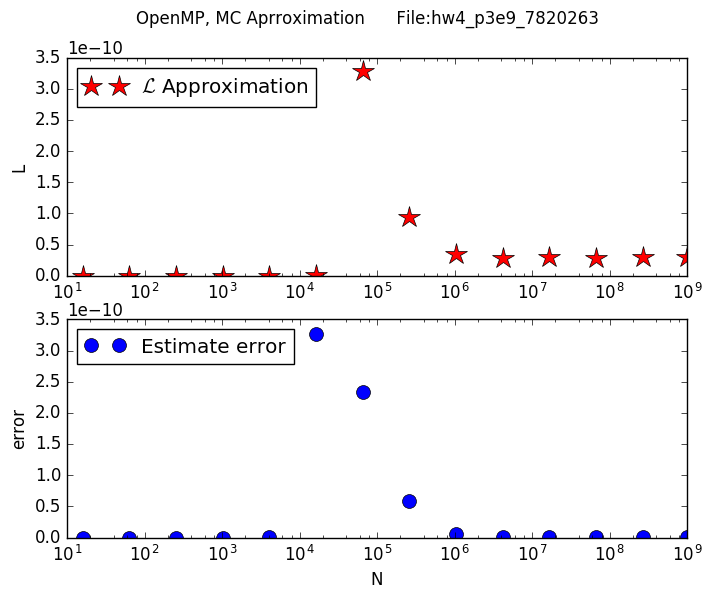
\includegraphics[width=0.8\textwidth]{hw4_p3e9_7820263.png}
	\end{center}
	\caption{Stampede Output}
	\label{fig:hw4_p3e9_7820263}
\end{figure}

Data for Fig.\ \ref{fig:hw4_p3e9_7820263}  which is created by C Program:\ref{fig:hw4_p3e9}  on Stampede, data files hw4\_p3e9\_7820263.stdou: 
\begin{lstlisting}
        16, 2.2835465291209360e-26 
        64, 2.9035855524601275e-18 
       256, 1.3789071769174436e-18 
      1024, 5.1856654013717579e-15 
      4096, 3.0222140530026563e-14 
     16384, 1.1384959333172844e-12 
     65536, 3.2803197641402003e-10 
    262144, 9.3953604238349840e-11 
   1048576, 3.4750342184101576e-11 
   4194304, 2.8930699656351799e-11 
  16777216, 2.9522543196705714e-11 
  67108864, 2.8097461616464975e-11 
 268435456, 2.9665714969964511e-11 
1000000000, 3.0307203895142228e-11 
\end{lstlisting}



\newpage
\textbf{\textit{Solution for Problem 3e
Satampede has a 2 hour time  limit and 16 node limit and I couldn't increase N for bigger iteratin.
I run the C code on my computer and got following info for bigger N iteration and generated following Fig:{ \ref{fig:hw4_p3e9_mycomputer} }   }} :

\begin{lstlisting}
 \end{lstlisting}


\begin{figure}[htb]
	\begin{center}
		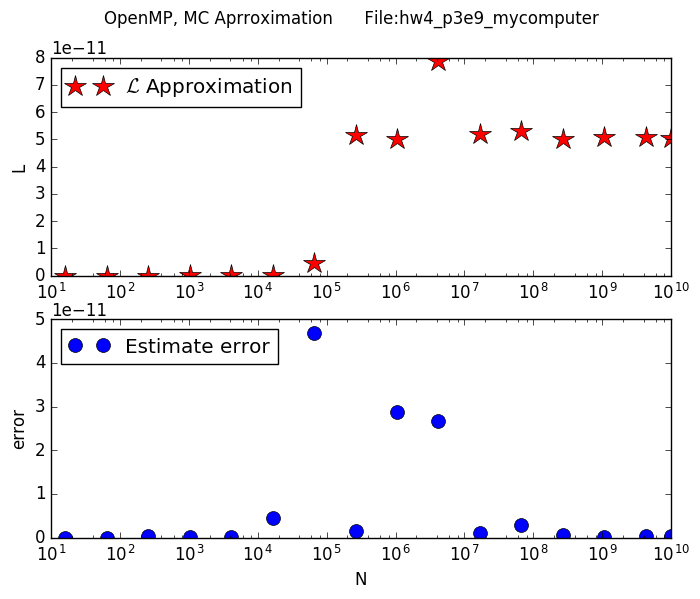
\includegraphics[width=0.8\textwidth]{hw4_p3e9_mycomputer.png}
	\end{center}
	\caption{Stampede Output}
	\label{fig:hw4_p3e9_mycomputer}
\end{figure}

Data for Fig:\ \ref{fig:hw4_p3e9_mycomputer}  which is created by C program above on my computer. Output files hw4\_p3e9\_mycomputer.stdou: 
\begin{lstlisting}
               16, 5.6806888452998559e-25 
               64, 1.4222922464502012e-19 
              256, 5.4809559857698940e-19 
             1024, 3.1772747368080066e-13 
             4096, 8.4128447079010768e-14 
            16384, 2.3113525609717192e-13 
            65536, 4.6925320908791665e-12 
           262144, 5.1593302333822248e-11 
          1048576, 5.0089050842028930e-11 
          4194304, 7.8744952751389459e-11 
         16777216, 5.1958906276835478e-11 
         67108864, 5.3031812887466585e-11 
        268435456, 5.0262984484768661e-11 
       1073741824, 5.0922160553917313e-11 
       4294967296, 5.0834543540211702e-11 
      10000000000, 5.0568383647416717e-11
               
                
\end{lstlisting}





\end{document}
